\documentclass[english,,doc,floatsintext]{apa6}
\usepackage{lmodern}
\usepackage{amssymb,amsmath}
\usepackage{ifxetex,ifluatex}
\usepackage{fixltx2e} % provides \textsubscript
\ifnum 0\ifxetex 1\fi\ifluatex 1\fi=0 % if pdftex
  \usepackage[T1]{fontenc}
  \usepackage[utf8]{inputenc}
\else % if luatex or xelatex
  \ifxetex
    \usepackage{mathspec}
  \else
    \usepackage{fontspec}
  \fi
  \defaultfontfeatures{Ligatures=TeX,Scale=MatchLowercase}
\fi
% use upquote if available, for straight quotes in verbatim environments
\IfFileExists{upquote.sty}{\usepackage{upquote}}{}
% use microtype if available
\IfFileExists{microtype.sty}{%
\usepackage{microtype}
\UseMicrotypeSet[protrusion]{basicmath} % disable protrusion for tt fonts
}{}
\usepackage{hyperref}
\hypersetup{unicode=true,
            pdftitle={Leave-one-out cross-validation for non-factorizable normal models},
            pdfauthor={Paul-Christian Bürkner, Jonah Gabry, \& Aki Vehtari},
            pdfkeywords={cross-validation, pareto-smoothed importance-sampling, non-factorizable
models, SAR models},
            pdfborder={0 0 0},
            breaklinks=true}
\urlstyle{same}  % don't use monospace font for urls
\ifnum 0\ifxetex 1\fi\ifluatex 1\fi=0 % if pdftex
  \usepackage[shorthands=off,main=english]{babel}
\else
  \usepackage{polyglossia}
  \setmainlanguage[]{english}
\fi
\usepackage{color}
\usepackage{fancyvrb}
\newcommand{\VerbBar}{|}
\newcommand{\VERB}{\Verb[commandchars=\\\{\}]}
\DefineVerbatimEnvironment{Highlighting}{Verbatim}{commandchars=\\\{\}}
% Add ',fontsize=\small' for more characters per line
\usepackage{framed}
\definecolor{shadecolor}{RGB}{248,248,248}
\newenvironment{Shaded}{\begin{snugshade}}{\end{snugshade}}
\newcommand{\AlertTok}[1]{\textcolor[rgb]{0.94,0.16,0.16}{#1}}
\newcommand{\AnnotationTok}[1]{\textcolor[rgb]{0.56,0.35,0.01}{\textbf{\textit{#1}}}}
\newcommand{\AttributeTok}[1]{\textcolor[rgb]{0.77,0.63,0.00}{#1}}
\newcommand{\BaseNTok}[1]{\textcolor[rgb]{0.00,0.00,0.81}{#1}}
\newcommand{\BuiltInTok}[1]{#1}
\newcommand{\CharTok}[1]{\textcolor[rgb]{0.31,0.60,0.02}{#1}}
\newcommand{\CommentTok}[1]{\textcolor[rgb]{0.56,0.35,0.01}{\textit{#1}}}
\newcommand{\CommentVarTok}[1]{\textcolor[rgb]{0.56,0.35,0.01}{\textbf{\textit{#1}}}}
\newcommand{\ConstantTok}[1]{\textcolor[rgb]{0.00,0.00,0.00}{#1}}
\newcommand{\ControlFlowTok}[1]{\textcolor[rgb]{0.13,0.29,0.53}{\textbf{#1}}}
\newcommand{\DataTypeTok}[1]{\textcolor[rgb]{0.13,0.29,0.53}{#1}}
\newcommand{\DecValTok}[1]{\textcolor[rgb]{0.00,0.00,0.81}{#1}}
\newcommand{\DocumentationTok}[1]{\textcolor[rgb]{0.56,0.35,0.01}{\textbf{\textit{#1}}}}
\newcommand{\ErrorTok}[1]{\textcolor[rgb]{0.64,0.00,0.00}{\textbf{#1}}}
\newcommand{\ExtensionTok}[1]{#1}
\newcommand{\FloatTok}[1]{\textcolor[rgb]{0.00,0.00,0.81}{#1}}
\newcommand{\FunctionTok}[1]{\textcolor[rgb]{0.00,0.00,0.00}{#1}}
\newcommand{\ImportTok}[1]{#1}
\newcommand{\InformationTok}[1]{\textcolor[rgb]{0.56,0.35,0.01}{\textbf{\textit{#1}}}}
\newcommand{\KeywordTok}[1]{\textcolor[rgb]{0.13,0.29,0.53}{\textbf{#1}}}
\newcommand{\NormalTok}[1]{#1}
\newcommand{\OperatorTok}[1]{\textcolor[rgb]{0.81,0.36,0.00}{\textbf{#1}}}
\newcommand{\OtherTok}[1]{\textcolor[rgb]{0.56,0.35,0.01}{#1}}
\newcommand{\PreprocessorTok}[1]{\textcolor[rgb]{0.56,0.35,0.01}{\textit{#1}}}
\newcommand{\RegionMarkerTok}[1]{#1}
\newcommand{\SpecialCharTok}[1]{\textcolor[rgb]{0.00,0.00,0.00}{#1}}
\newcommand{\SpecialStringTok}[1]{\textcolor[rgb]{0.31,0.60,0.02}{#1}}
\newcommand{\StringTok}[1]{\textcolor[rgb]{0.31,0.60,0.02}{#1}}
\newcommand{\VariableTok}[1]{\textcolor[rgb]{0.00,0.00,0.00}{#1}}
\newcommand{\VerbatimStringTok}[1]{\textcolor[rgb]{0.31,0.60,0.02}{#1}}
\newcommand{\WarningTok}[1]{\textcolor[rgb]{0.56,0.35,0.01}{\textbf{\textit{#1}}}}
\usepackage{graphicx,grffile}
\makeatletter
\def\maxwidth{\ifdim\Gin@nat@width>\linewidth\linewidth\else\Gin@nat@width\fi}
\def\maxheight{\ifdim\Gin@nat@height>\textheight\textheight\else\Gin@nat@height\fi}
\makeatother
% Scale images if necessary, so that they will not overflow the page
% margins by default, and it is still possible to overwrite the defaults
% using explicit options in \includegraphics[width, height, ...]{}
\setkeys{Gin}{width=\maxwidth,height=\maxheight,keepaspectratio}
\IfFileExists{parskip.sty}{%
\usepackage{parskip}
}{% else
\setlength{\parindent}{0pt}
\setlength{\parskip}{6pt plus 2pt minus 1pt}
}
\setlength{\emergencystretch}{3em}  % prevent overfull lines
\providecommand{\tightlist}{%
  \setlength{\itemsep}{0pt}\setlength{\parskip}{0pt}}
\setcounter{secnumdepth}{5}
% Redefines (sub)paragraphs to behave more like sections
\ifx\paragraph\undefined\else
\let\oldparagraph\paragraph
\renewcommand{\paragraph}[1]{\oldparagraph{#1}\mbox{}}
\fi
\ifx\subparagraph\undefined\else
\let\oldsubparagraph\subparagraph
\renewcommand{\subparagraph}[1]{\oldsubparagraph{#1}\mbox{}}
\fi

%%% Use protect on footnotes to avoid problems with footnotes in titles
\let\rmarkdownfootnote\footnote%
\def\footnote{\protect\rmarkdownfootnote}


  \title{Leave-one-out cross-validation for non-factorizable normal models}
    \author{Paul-Christian Bürkner\textsuperscript{1}, Jonah
Gabry\textsuperscript{2}, \& Aki Vehtari\textsuperscript{3}}
    \date{}
  
\shorttitle{Cross-validation for non-factorizable models}
\affiliation{
\vspace{0.5cm}
\textsuperscript{1} Department of Psychology, University of Münster, Germany\\\textsuperscript{2} Institute for Social and Economic Research in Policy, Columbia University, USA\\\textsuperscript{3} Department of Computer Science, Aalto University, Finland}
\keywords{cross-validation, pareto-smoothed importance-sampling, non-factorizable models, SAR models}
\usepackage{csquotes}
\usepackage{upgreek}
\captionsetup{font=singlespacing,justification=justified}

\usepackage{longtable}
\usepackage{lscape}
\usepackage{multirow}
\usepackage{tabularx}
\usepackage[flushleft]{threeparttable}
\usepackage{threeparttablex}

\newenvironment{lltable}{\begin{landscape}\begin{center}\begin{ThreePartTable}}{\end{ThreePartTable}\end{center}\end{landscape}}

\makeatletter
\newcommand\LastLTentrywidth{1em}
\newlength\longtablewidth
\setlength{\longtablewidth}{1in}
\newcommand{\getlongtablewidth}{\begingroup \ifcsname LT@\roman{LT@tables}\endcsname \global\longtablewidth=0pt \renewcommand{\LT@entry}[2]{\global\advance\longtablewidth by ##2\relax\gdef\LastLTentrywidth{##2}}\@nameuse{LT@\roman{LT@tables}} \fi \endgroup}


\usepackage{lineno}

\linenumbers
\usepackage{mathtools}
\usepackage[utf8]{inputenc}
\usepackage[T1]{fontenc}
\usepackage{textcomp}
\usepackage{graphicx,pdflscape}
\usepackage{geometry}
\usepackage{amsmath}
\usepackage{float}
\usepackage{supertabular}
\usepackage{booktabs,caption,fixltx2e}
\usepackage[flushleft]{threeparttable}
\usepackage{natbib}
\usepackage{tcolorbox}
\usepackage{paralist}
\usepackage{multicol}
\newcommand\numberthis{\addtocounter{equation}{1}\tag{\theequation}}

\authornote{

Correspondence concerning this article should be addressed to Aki
Vehtari, Department of Computer Science, Aalto University, Finland.
E-mail:
\href{mailto:Aki.Vehtari@aalto.fi}{\nolinkurl{Aki.Vehtari@aalto.fi}}}

\abstract{
Cross-validation can be used to measure a models predictive accuracy for
instance for the purpose of model comparison or selection. As exact
cross-validation is often practically infeasible for Bayesian models
because it requires too much time, approximate cross-validation methods
have been developed; most notably methods for leave-one-out
cross-validation (LOO-CV). However, standard LOO-CV requires the
likelihood to be factorizable, that is the observations have to be
conditionally independent given the model parameters. Unfortunately,
some important statistical models most notably in the context of
temporal and spatial statistics are non-factorizable, but LOO-CV may
still be an important measure for these models. For this reason, we
derive how to compute and validate exact and approximate LOO-CV for
non-factorizable models that follow a multivariate normal likelhood.


}

\usepackage{amsthm}
\newtheorem{theorem}{Theorem}[section]
\newtheorem{lemma}{Lemma}[section]
\theoremstyle{definition}
\newtheorem{definition}{Definition}[section]
\newtheorem{corollary}{Corollary}[section]
\newtheorem{proposition}{Proposition}[section]
\theoremstyle{definition}
\newtheorem{example}{Example}[section]
\theoremstyle{definition}
\newtheorem{exercise}{Exercise}[section]
\theoremstyle{remark}
\newtheorem*{remark}{Remark}
\newtheorem*{solution}{Solution}
\begin{document}
\maketitle

\hypertarget{introduction}{%
\section{Introduction}\label{introduction}}

After fitting a statistical model, we often want to measure its
predictive accuracy, for instance for the purpose of model comparison or
selection (Ando \& Tsay, 2010; Geisser \& Eddy, 1979; Vehtari \&
Lampinen, 2002; Vehtari, Ojanen, \& others, 2012). In the absence of
actual new data to predict, one general approach to evaluating a model's
predictive accuracy is cross-validation (Vehtari \& Lampinen, 2002).
When doing cross-validation, the data is split into two subsets. Based
on the first subset we fit the statistical model and then evaluate its
predictive accuarcy for the second subset. We may do this once or many
times each time leaving out another subset.

One widely applied type of cross-validation is \emph{leave-one-out
cross-validation} (LOO-CV), where each time a single observation is left
out and then predicted based on the model fit to the remaining data
(Vehtari et al., 2017b). Predictive accuarcy is evaluated by first
computing the expected log predictive density of the left-out
observation and then taking the sum of these values over all
observations to obtain the expected log predictive density as a single
measure of predictive accuracy. Unfortunately, exact LOO-CV is costly as
it requires to fit the model as many times are there are observations in
the data. Depending on the size of the data, complexity of the model,
and estimation method, this can be practically infeasible as it simply
requires too much time (Vehtari et al., 2017b). For this reason,
approximate versions of LOO-CV have been developed, most notably
approximations via Pareto-smoothed importance-sampling (PSIS-LOO-CV;
Vehtari et al., 2017b, 2017a), which is applicable to Bayesian models.

A standard assumption of any such LOO-CV approach is that the joint
likelihood of the model over all observations has to be factorizable,
that is the observations have to be pairwise conditionally independent
given the model parameters. The purpose of the present paper is to
generalize PSIS-LOO-CV to non-factorized or non-factorizable models
where observations are dependent even after conditioning on the model
parameters.

\hypertarget{approximate-loo-cv-using-integrated-importance-sampling}{%
\subsection{Approximate LOO-CV using integrated
importance-sampling}\label{approximate-loo-cv-using-integrated-importance-sampling}}

We start by introducing the mathematical basis of approximative LOO-CV.
We index observations by \(i\) and denote the corresponding response
value by \(y_i\). Further, we use \(y\) to indicate the response vector
of all observations and \(y_{-i}\) to indicate the response vector
without the \(i\)th value. Model parameters are referred to as
\(\theta\). Throughout, a Bayesian model specification and estimation
via Markov-Chain Monte-Carlo (MCMC) methods is assumed. To obtain the
leave-one-out predictive density \(p(y_i \,|\, y_{-i})\) we need to
integrate over \(\theta\):

\begin{equation}
p(y_i\,|\,y_{-i}) =
  \int p(y_i\,|\, y_{-i}, \theta) \, p(\theta\,|\, y_{-i}) \,d \theta.
\end{equation}

Here, \(p(\theta\,|\, y_{-i})\) is the leave-one-out posterior
distribution for \(\theta\), that is, the posterior distribution for
\(\theta\) obtained by fitting the model while holding out the \(i\)th
observation.

To avoid the cost of sampling from \(N\) leave-one-out posteriors, it is
possible to take the posterior draws \(\theta^{(s)}\)
\((s=1,\ldots,S)\), from the \emph{full} posterior \(p(\theta\,|\, y)\),
and then approximate the above integral using integrated importance
sampling (see Section 3.6.1 in Vehtari, Mononen, Tolvanen, Sivula, \&
Winther, 2016):

\begin{equation}
 p(y_i\,|\, y_{-i}) \approx
   \frac{ \sum_{s=1}^S p(y_i\,|\,y_{-i},\,\theta^{(s)}) \,w_i^{(s)}}{ \sum_{s=1}^S w_i^{(s)}}
\end{equation}

In the above euquation, \(w_i^{(s)}\) are importance weights to be
computed as follows. First we compute the raw importance ratios

\begin{equation}
  r_i^{(s)} \propto \frac{1}{p(y_i \,|\, y_{-i}, \, \theta^{(s)})},
\end{equation}

and then stabilize them using Pareto smoothed importance sampling to
obtain the weights \(w_i^{(s)}\) (Vehtari et al., 2017b, 2017a). The
resulting approximation is referred to as PSIS-LOO-CV (Vehtari et al.,
2017b).

\hypertarget{nf-loo-cv}{%
\section{Leave-one-out cross validation for non-factorizable
models}\label{nf-loo-cv}}

When computing approximate LOO-CV after fitting a Bayesian model, the
first step is to calculate the \emph{pointwise} log-likelihood for every
response value \(y_i, \: i = 1, \ldots, N\). This is straightforward for
\emph{factorizable} models in which response values are conditionally
independent given the model parameters \(\theta\) and the likelihood can
be written in the familiar form

\begin{equation}
p(y \,|\, \theta) = \prod_{i=1}^N p(y_i \,|\, \theta).
\end{equation}

The function \(p\) will be either a probability density function (PDF)
or a probability mass function (PMF) depending on whether we have a
continuous or discrete outcome. When \(p(y)\) can be factorized in this
way, the conditional pointwise log-likelihood can be obtained easily by
computing \(\log p(y_i \,|\, \theta)\) for each \(i\). We then save each
of these individual contributions to the log-likelihood rather than
simply summing them to obtain the total log-likelihood.

The situation is more complicated for \emph{non-factorizable} models in
which response values are not conditionally independent. When there is
residual dependency even after accounting for the model parameters
\(\theta\), the conditional pointwise log-likelihood has the general
form \(\log p(y_i \,|\, y_{-i}, \theta)\), where, again, \(y_{-i}\)
denotes all response values except observation \(i\).

\hypertarget{loo-cv-for-multivariate-normal-models}{%
\subsection{LOO-CV for multivariate normal
models}\label{loo-cv-for-multivariate-normal-models}}

Although computing the pointwise log-likelihood for non-factorizable
models is often impossible, there is a large class of multivariate
normal models for which an analytical solution is available. These
equations were initially derived by Sundararajan and Keerthi (2001) with
a focus on the special case of a zero-mean Gaussian process model with
prior covariance \(K\) and residual standard deviation \(\sigma\),

\begin{equation}
y \sim {\mathrm N}(0, \, K+\sigma^2 I),
\end{equation}

where \(I\) is the identity matrix of appropriate dimension and
\(C = K+\sigma^2 I\) is the covariance matrix of the model. Sundararajan
and Keerthi's derivations make no use of the special form of \(C\) for
Gaussian process models and thus immediately generalize to the case of
an arbitrary invertible covariance matrix \(C\). For such models, the
LOO predictive mean and standard deviation can be computed as follows:

\begin{align}
\label{ypredpars}
  \mu_{\tilde{y},-i} &= y_i-\bar{c}_{ii}^{-1} g_i \nonumber \\
  \sigma_{\tilde{y},-i} &= \sqrt{\bar{c}_{ii}^{-1}},
\end{align}

where \(g_i = \left[C^{-1} y\right]_i\) and
\(\bar{c}_{ii} = \left[C^{-1}\right]_{ii}\). The log predictive density
of the \(i\)th observation is then computed as

\begin{equation}
  \log p(y_i \,|\, y_{-i},\theta)
  = - \frac{1}{2}\log(2\pi)
  - \frac{1}{2}\log \sigma^2_{-i}
  - \frac{1}{2}\frac{(y_i-\mu_{-i})^2}{\sigma^2_{-i}}.
\end{equation}

Expressing this same equation in terms of \(g_i\) and \(\bar{c}_{ii}\),
the log predictive density becomes:

\begin{equation}
  \log p(y_i \,|\, y_{-i},\theta)
  = - \frac{1}{2}\log(2\pi)
  + \frac{1}{2}\log \bar{c}_{ii}
  - \frac{1}{2}\frac{g_i^2}{\bar{c}_{ii}}
\end{equation}

(note that Vehtari et al. (2016) has a typo in the corresponding
Equation 34). From these equations we can now derive a recipe for
obtaining the conditional pointwise log-likelihood for \emph{all} models
that can be expressed conditionally in terms of a multivariate normal
with invertible covariance matrix \(C\).

\hypertarget{exact-loo-cv-with-re-fitting}{%
\subsection{Exact LOO-CV with
re-fitting}\label{exact-loo-cv-with-re-fitting}}

In order to validate the approximate LOO-CV procedure, and also in order
to allow exact computations to be made for a small number of
leave-one-out folds for which the Pareto \(k\) diagnostic (Vehtari et
al., 2017a) indicates an unstable approximation, we need to consider how
we might to do \emph{exact} LOO-CV for a non-factorizable model. In the
case of a Gaussian process that has the marginalization property, we
could just drop the one row and column of \(C\) corresponding to the
held out out observation. This does not hold in general for multivariate
normal models, however, and to keep the original prior we may need to
maintain the full covariance matrix \(C\) even when one of the
observations is left out.

The solution is to model \(y_i\) as a missing observation and estimate
it along with all of the other model parameters. For a conditional
multivariate normal model, \(\log p(y_i\,|\,y_{-i})\) can be computed as
follows. First, we model \(y_i\) as missing and denote the corresponding
parameter \(y_i^{\mathrm{mis}}\). Then, we define

\begin{equation}
y_{\mathrm{mis}(i)} = (y_1, \ldots, y_{i-1}, y_i^{\mathrm{mis}}, y_{i+1}, \ldots, y_N).
\end{equation}

to be the same as the full set of observations \(y\), except replacing
\(y_i\) with the parameter \(y_i^{\mathrm{mis}}\).

Second, we compute the LOO predictive mean and standard deviations as
above, but replace \(y\) with \(y_{\mathrm{mis}(i)}\) in the computation
of \(\mu_{\tilde{y},-i}\):

\begin{equation}
\mu_{\tilde{y},-i} = y_{{\mathrm{mis}}(i)}-\bar{c}_{ii}^{-1}g_i,
\end{equation}

where in this case we have

\begin{equation}
g_i = \left[ C^{-1} y_{\mathrm{mis}(i)} \right]_i.
\end{equation}

The conditional log predictive density is then computed with the above
\(\mu_{\tilde{y},-i}\) and the left out observation \(y_i\):

\begin{equation}
  \log p(y_i\,|\,y_{-i},\theta)
  = - \frac{1}{2}\log(2\pi)
  - \frac{1}{2}\log \sigma^2_{\tilde{y},-i}
  - \frac{1}{2}\frac{(y_i-\mu_{\tilde{y},-i})^2}{\sigma^2_{\tilde{y},-i}}.
\end{equation}

Finally, the leave-one-out predictive distribution can then be estimated
as

\begin{equation}
 p(y_i\,|\,y_{-i}) \approx \frac{1}{S} \sum_{s=1}^S p(y_i\,|\,y_{-i}, \theta_{-i}^{(s)}),
\end{equation}

where \(\theta_{-i}^{(s)}\) are draws from the posterior distribution
\(p(\theta\,|\,y_{\mathrm{mis}(i)})\).

\hypertarget{case-study}{%
\section{Case Study}\label{case-study}}

A common non-factorizable multivariate normal model is the
simultaneously autoregressive (SAR) model, which is frequently used for
spatially correlated data. The lagged SAR model is defined as

\begin{equation}
y = \rho Wy + \eta + \epsilon
\end{equation}

or equivalently

\begin{equation}
(I - \rho W)y = \eta + \epsilon,
\end{equation}

where \(\rho\) is the spatial correlation parameter and \(W\) is a
user-defined weight matrix. The matrix \(W\) has entries \(w_{ii} = 0\)
along the diagonal and the off-diagonal entries \(w_{ij}\) are larger
when areas \(i\) and \(j\) are closer to each other. In a linear model,
the predictor term \(\eta\) is given by \(\eta = X \beta\) with design
matrix \(X\) and regression coefficients \(\beta\). However, since the
above equation holds for arbitrary \(\eta\), these results are not
restricted to linear models. If we have
\(\epsilon \sim {\mathrm N}(0, \,\sigma^2 I)\), it follows that

\begin{equation}
(I - \rho W)y \sim {\mathrm N}(\eta, \sigma^2 I).
\end{equation}

For the purpose of computing LOO-CV, it makes sense to rewrite the SAR
model in slightly different form. Conditional on \(\rho\), \(\eta\), and
\(\sigma\), if we write

\begin{equation}
y-(I-\rho W)^{-1}\eta \sim {\mathrm N}(0, \sigma^2(I-\rho W)^{-1}(I-\rho W)^{-T}),
\end{equation}

or more compactly, with \(\widetilde{W}=(I-\rho W)\),

\begin{equation}
y-\widetilde{W}^{-1}\eta \sim {\mathrm N}(0, \sigma^2(\widetilde{W}^{T}\widetilde{W})^{-1}),
\end{equation}

then this has the same form as the zero mean Gaussian process from
above. Accordingly, we can compute the leave-one-out predictive
densities with the equations from Sundararajan and Keerthi (2001),
replacing \(y\) with \((y-\widetilde{W}^{-1}\eta)\) and taking the
covariance matrix \(C\) to be
\(\sigma^2(\widetilde{W}^{T}\widetilde{W})^{-1}\).

\hypertarget{neighborhood-crime-in-columbus-ohio}{%
\subsubsection{Neighborhood Crime in Columbus,
Ohio}\label{neighborhood-crime-in-columbus-ohio}}

In order to demonstrate how to carry out the computations implied by
these equations, we will first fit a lagged SAR model to data on crime
in 49 different neighborhoods of Columbus, Ohio during the year 1980.
The data was originally described in Anselin (1988) and ships with the
spdep package (Bivand \& Piras, 2015).

In addition to the loo package (Vehtari, Gelman, \& Gabry, 2018), for
this analysis we use the brms interface (Bürkner, 2017, 2018) to Stan
(Carpenter et al., 2017) to generate a Stan program and fit the model,
and also the bayesplot (Gabry \& Mahr, 2018) and ggplot2 (Wickham, 2016)
packages for plotting. The three variables in the data set relevant to
this example are: \texttt{CRIME}: the number of residential burglaries
and vehicle thefts per thousand households in the neighbood,
\texttt{HOVAL}: housing value in units of \$1000 USD, and \texttt{INC}:
household income in units of \$1000 USD. We will also use the object
\texttt{COL.nb}, which is a list containing information about which
neighborhoods border each other. From this list we will be able to
construct the weight matrix to used to help account for the spatial
dependency among the observations. The complete R code for this case
study can be found at
(\url{http://mc-stan.org/loo/articles/loo2-non-factorizable.html}).

A model predicting \texttt{CRIME} from \texttt{INC} and \texttt{HOVAL},
while accounting for the spatial dependency via an SAR structure, can be
specified in brms as follows:

\begin{Shaded}
\begin{Highlighting}[]
\KeywordTok{brm}\NormalTok{(CRIME }\OperatorTok{~}\StringTok{ }\NormalTok{INC }\OperatorTok{+}\StringTok{ }\NormalTok{HOVAL, }\DataTypeTok{data =}\NormalTok{ COL.OLD, }\DataTypeTok{autocor =} \KeywordTok{cor_lagsar}\NormalTok{(COL.nb))}
\end{Highlighting}
\end{Shaded}

In Figure \ref{fig:plot-lagsar}, we see that both higher income and
higher housing value predict lower crime rates in the neighborhood.
Moreover, there seems to be substantial spatial correlation between
adjacent neighborhoods, as indicated by the posterior distribution of
the \texttt{lagsar} parameter.

\begin{figure}
\centering
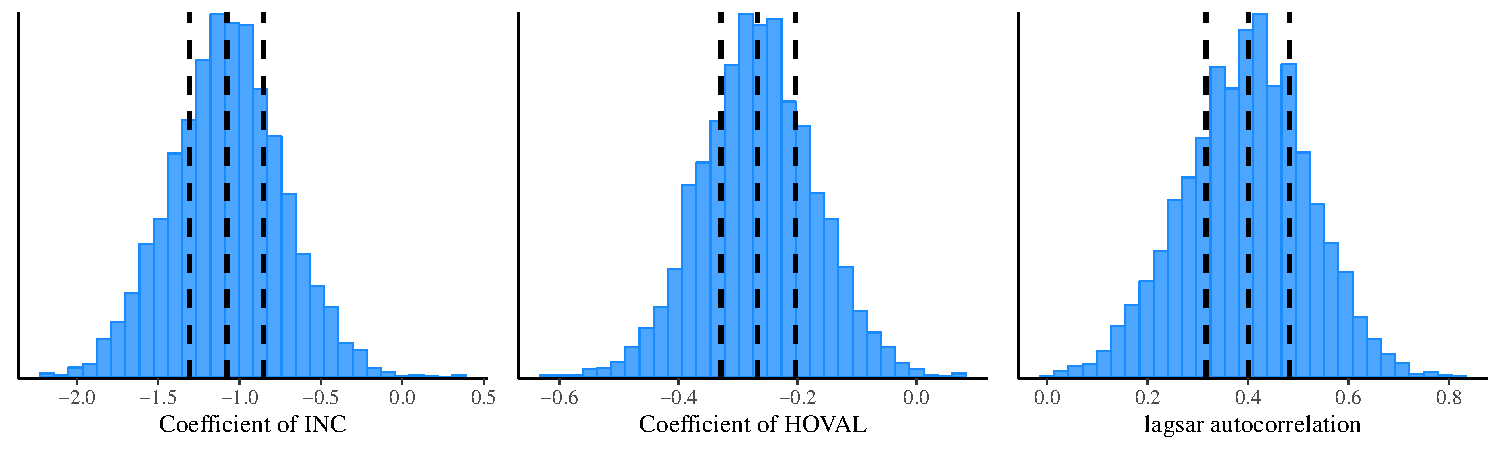
\includegraphics{psis_non_factorizable_models_files/figure-latex/plot-lagsar-1.pdf}
\caption{\label{fig:plot-lagsar}Posterior distribution of selected
parameters of the lagged SAR model along with posterior median and 50\%
central interval.}
\end{figure}

\hypertarget{approximate-and-exact-loo-cv}{%
\subsubsection{Approximate and exact
LOO-CV}\label{approximate-and-exact-loo-cv}}

After fitting the model, the next step is to compute the pointwise
log-likelihood values needed for approximate LOO-CV. To do this we use
the recipe laid out in Section \ref{nf-loo-cv}.

The quality of the PSIS-LOO approximation can be investigated
graphically by plotting the Pareto-k estimate for each observation.
Ideally, they should not exceed \(0.5\), but in practice the algorithm
turns out to be robust up to values of \(0.7\) (Vehtari et al., 2017b,
2017a). In Figure \ref{fig:psis-res-nb}, we see that the fourth
observation is problematic and so may reduce the accuracy of the LOO-CV
approximation.

\begin{figure}
\centering
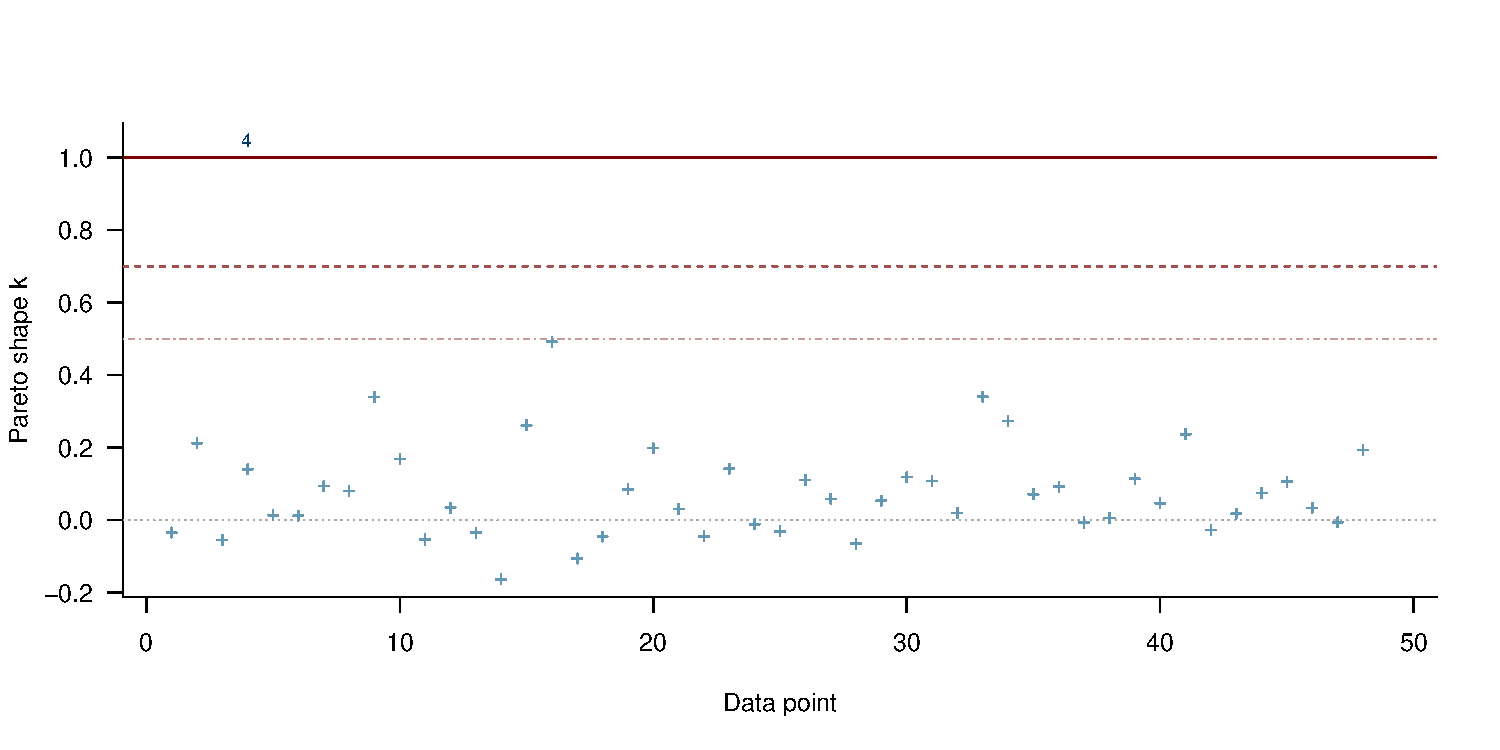
\includegraphics{psis_non_factorizable_models_files/figure-latex/psis-res-nb-1.pdf}
\caption{\label{fig:psis-res-nb}PSIS diagnostic plot showing the
Pareto-k-estimate of each observation.}
\end{figure}

The PSIS-LOO-CV to approximation of the expected log predictive density
for new data reveals \(\text{elpd}_{\text{approx}} =\) -187.25. This
result still needs to be validated against exact LOO-CV, which is
somewhat more involved, as we need to re-fit the model \(N\) times each
time leaving out a single observations. For the lagged SAR model, we
cannot just ignore the held-out observation entirely as this will change
the prior of the other observations. In other words, the lagged SAR
model does not have the marginalization property that holds, for
instance, for Gaussian process models. Instead, we have to model the
held-out observation as a missing value, which is to be estimated along
with the other model parameters (see
\url{http://mc-stan.org/loo/articles/loo2-non-factorizable.html} for
details on the R code).

A first step in the validation of the pointwise predictive density is to
compare the distribution of the implied response values for the left-out
observation using the pointwise mean and standard deviation from
(\ref{ypredpars}) to the distribution of the \(y_i^{\mathrm{mis}}\)
posterior-predictive values estimated as part of the model. If the
pointwise predictive density is correct, the two distributions should
match very closely (up to sampling error). In Figure \ref{fig:yplots},
we overlay these two distributions for the first four observations and
see that they match very closely (as is the case for all \(49\)
observations of in this example).

\begin{figure}
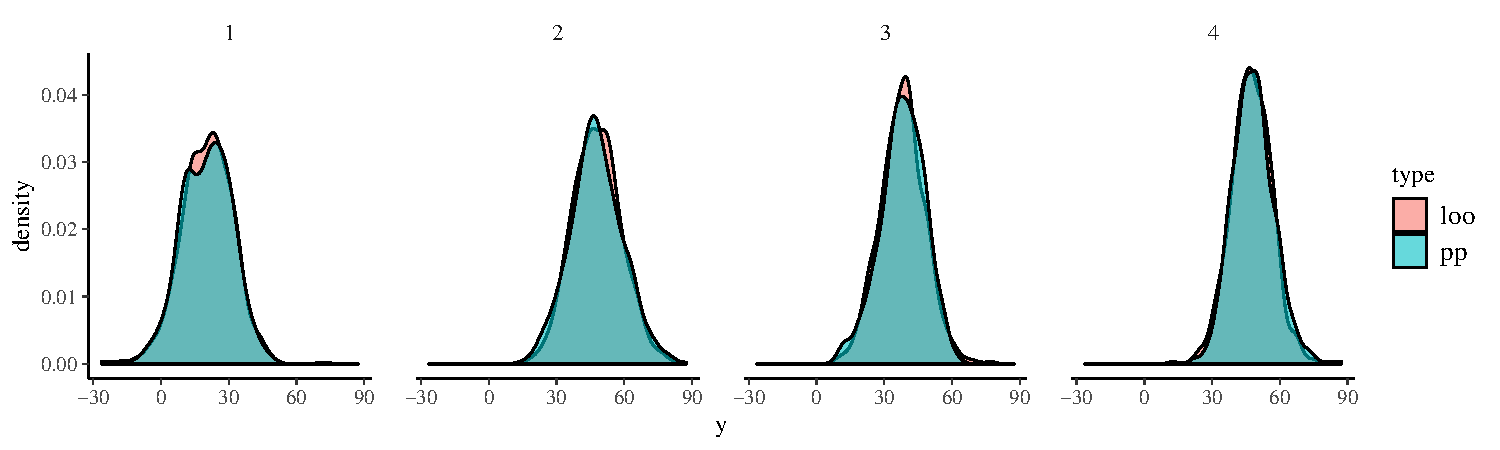
\includegraphics[width=0.95\linewidth]{psis_non_factorizable_models_files/figure-latex/yplots-1} \caption{Implied response values of the first four observations computed (a) after model fitting (type = 'loo') and (b) as part of the model in the form of posterior-predictive draws (type = 'pp').}\label{fig:yplots}
\end{figure}

In the final step, we compute the pointwise predictive density based on
the exact LOO-CV and compare it to the approximate PSIS-LOO-CV result
computed earlier. The results of the approximate
(\(\text{elpd}_{\text{approx}} =\) -187.25) and exact LOO-CV
(\(\text{elpd}_{\text{exact}} =\) -188.32) are similar but not as close
as we would expect if there were no problematic observations. We can
investigate this issue more closely by plotting the approximate against
the exact pointwise ELPD values.

\begin{figure}
\centering
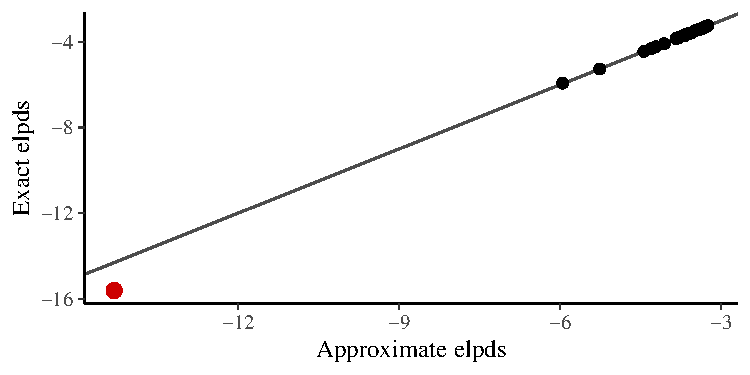
\includegraphics{psis_non_factorizable_models_files/figure-latex/elpd-compare-1.pdf}
\caption{\label{fig:elpd-compare}Comparison of approximate and exact
pointwise elpd values for the SAR model. Problematic observations are
marked as red dots.}
\end{figure}

In Figure \ref{fig:elpd-compare}, the fourth data point -- the
observation flagged as problematic by the PSIS-LOO approximation -- is
colored in red and is the clear outlier. Otherwise, the correspondence
between the exact and approximate values is strong. In fact, summing
over the pointwise ELPD values and leaving out the fourth observation
yields practically equivalent results for approximate and exact LOO-CV
(\(\text{elpd}_{\text{approx},-4} =\) -172.94 vs.
\(\text{elpd}_{\text{exact},-4} =\) -173.00). From this we can conclude
that the difference we found when including \emph{all} observations does
not indicate an error in the implementation of the approximate LOO-CV
but rather a violation of its assumptions.

\hypertarget{conclusion}{%
\section{Conclusion}\label{conclusion}}

In summary, we have shown how to set up and validate approximate and
exact LOO-CV for non-factorizable multivariate normal models. We
demonstrated the usefulness of our approach with a case study involving
the non-factorizable spatial SAR model. Although we motivated the
present paper by means of non-factorizable models (i.e.~models that
cannot be factorized at all), we note that our approach also works for
any Bayesian model that can be expressed in terms of a multivariate
normal likelihood. That is, we can also apply it to models that are
factorizable but for which the factorized representation is difficult to
compute or not available to the researcher for some other reasons.

\hypertarget{references}{%
\section*{References}\label{references}}
\addcontentsline{toc}{section}{References}

\hypertarget{refs}{}
\leavevmode\hypertarget{ref-ando2010}{}%
Ando, T., \& Tsay, R. (2010). Predictive likelihood for bayesian model
selection and averaging. \emph{International Journal of Forecasting},
\emph{26}(4), 744--763.

\leavevmode\hypertarget{ref-anselin1988}{}%
Anselin, L. (1988). \emph{Spatial econometrics: Methods and models}.
Dordrecht: Kluwer Academic.

\leavevmode\hypertarget{ref-bivand2015}{}%
Bivand, R., \& Piras, G. (2015). Comparing implementations of estimation
methods for spatial econometrics. \emph{Journal of Statistical
Software}, \emph{63}(18), 1--36. Retrieved from
\url{http://www.jstatsoft.org/v63/i18/}

\leavevmode\hypertarget{ref-brms1}{}%
Bürkner, P.-C. (2017). brms: An R package for bayesian multilevel models
using Stan. \emph{Journal of Statistical Software}, \emph{80}(1), 1--28.
doi:\href{https://doi.org/10.18637/jss.v080.i01}{10.18637/jss.v080.i01}

\leavevmode\hypertarget{ref-brms2}{}%
Bürkner, P.-C. (2018). Advanced bayesian multilevel modeling with the R
package brms. \emph{The R Journal}, 395--411. Retrieved from
\url{https://journal.r-project.org/archive/2018/RJ-2018-017}

\leavevmode\hypertarget{ref-carpenter2017}{}%
Carpenter, B., Gelman, A., Hoffman, M., Lee, D., Goodrich, B.,
Betancourt, M., \ldots{} Ridell, A. (2017). Stan: A probabilistic
programming language. \emph{Journal of Statistical Software}.

\leavevmode\hypertarget{ref-bayesplot}{}%
Gabry, J., \& Mahr, T. (2018). \emph{Bayesplot: Plotting for bayesian
models}. Retrieved from
\url{https://CRAN.R-project.org/package=bayesplot}

\leavevmode\hypertarget{ref-geisser1979}{}%
Geisser, S., \& Eddy, W. F. (1979). A predictive approach to model
selection. \emph{Journal of the American Statistical Association},
\emph{74}(365), 153--160.

\leavevmode\hypertarget{ref-sundararajan2001}{}%
Sundararajan, S., \& Keerthi, S. S. (2001). Predictive approaches for
choosing hyperparameters in gaussian processes. \emph{Neural
Computation}, \emph{13}(5), 1103--1118.

\leavevmode\hypertarget{ref-vehtari2017psis}{}%
Vehtari, A., Gelman, A., \& Gabry, J. (2017a). Pareto smoothed
importance sampling. \emph{arXiv Preprint}. Retrieved from
\url{https://arxiv.org/abs/1507.02646}

\leavevmode\hypertarget{ref-vehtari2017loo}{}%
Vehtari, A., Gelman, A., \& Gabry, J. (2017b). Practical bayesian model
evaluation using leave-one-out cross-validation and waic.
\emph{Statistics and Computing}, \emph{27}(5), 1413--1432. Retrieved
from \url{http://link.springer.com/article/10.1007/s11222-016-9696-4}

\leavevmode\hypertarget{ref-loo2018}{}%
Vehtari, A., Gelman, A., \& Gabry, J. (2018). \emph{loo: Efficient
leave-one-out cross-validation and WAIC for Bayesian models.} Retrieved
from \url{https://github.com/stan-dev/loo}

\leavevmode\hypertarget{ref-vehtari2002}{}%
Vehtari, A., \& Lampinen, J. (2002). Bayesian model assessment and
comparison using cross-validation predictive densities. \emph{Neural
Computation}, \emph{14}(10), 2439--2468.

\leavevmode\hypertarget{ref-vehtari2016}{}%
Vehtari, A., Mononen, T., Tolvanen, V., Sivula, T., \& Winther, O.
(2016). Bayesian leave-one-out cross-validation approximations for
gaussian latent variable models. \emph{Journal of Machine Learning
Research}, \emph{17}(103), 1--38. Retrieved from
\url{http://jmlr.org/papers/v17/14-540.html}

\leavevmode\hypertarget{ref-vehtari2012}{}%
Vehtari, A., Ojanen, J., \& others. (2012). A survey of bayesian
predictive methods for model assessment, selection and comparison.
\emph{Statistics Surveys}, \emph{6}, 142--228.

\leavevmode\hypertarget{ref-ggplot2}{}%
Wickham, H. (2016). \emph{Ggplot2: Elegant graphics for data analysis}.
Springer-Verlag New York. Retrieved from \url{http://ggplot2.org}


\end{document}
